The Large Hadron Collider (LHC) \cite{2008.LHC} is the most powerful particle accelerator in the world, colliding two beams of protons at a center of mass energy of \com{13}.
It is operated by the European Organization for Nuclear Research (CERN) and consists of a 27~km ring located beneath the France--Switzerland border.
A chain of smaller accelerators incrementally boost the protons\footnote{The LHC can also collide beams of heavy ions; however, this thesis focuses exclusively on the proton-proton collisions.} up to higher and higher energies before they reach the final collision energy within the main LHC ring.
Collisions occur at each of four detector experiments situated around the ring: ATLAS~\cite{PERF-2007-01}, ALICE~\cite{2008.alice}, CMS~\cite{2008.cms}, and LHCb~\cite{2008.lhcb}.

Protons are obtained from hydrogen atoms stripped of their electrons by an electric field.
A beam of protons is first accelerated up to $50\mev$ in the Linac 2 accelerator, then to $1.4\gev$ in the Proton Synchroton Booster (PSB), $25\gev$ in the Proton Synchrotron (PS), and finally to $450\gev$ in the Super Proton Synchrotron (SPS).
They are then injected into the LHC ring in two beams running in opposite directions where they accelerate up to the collision energy of $6.5\tev$.
The beams consist of bunches containing on the order of $10^{11}$ protons separated by $25~\textrm{ns}$~\cite{2019.accelerator-complex}.
A schematic of the CERN accelerator complex, including the chain of accelerators mentioned above, is shown in Figure~\ref{fig:detector_accelerator_complex}.

\begin{figure}
  \centering
  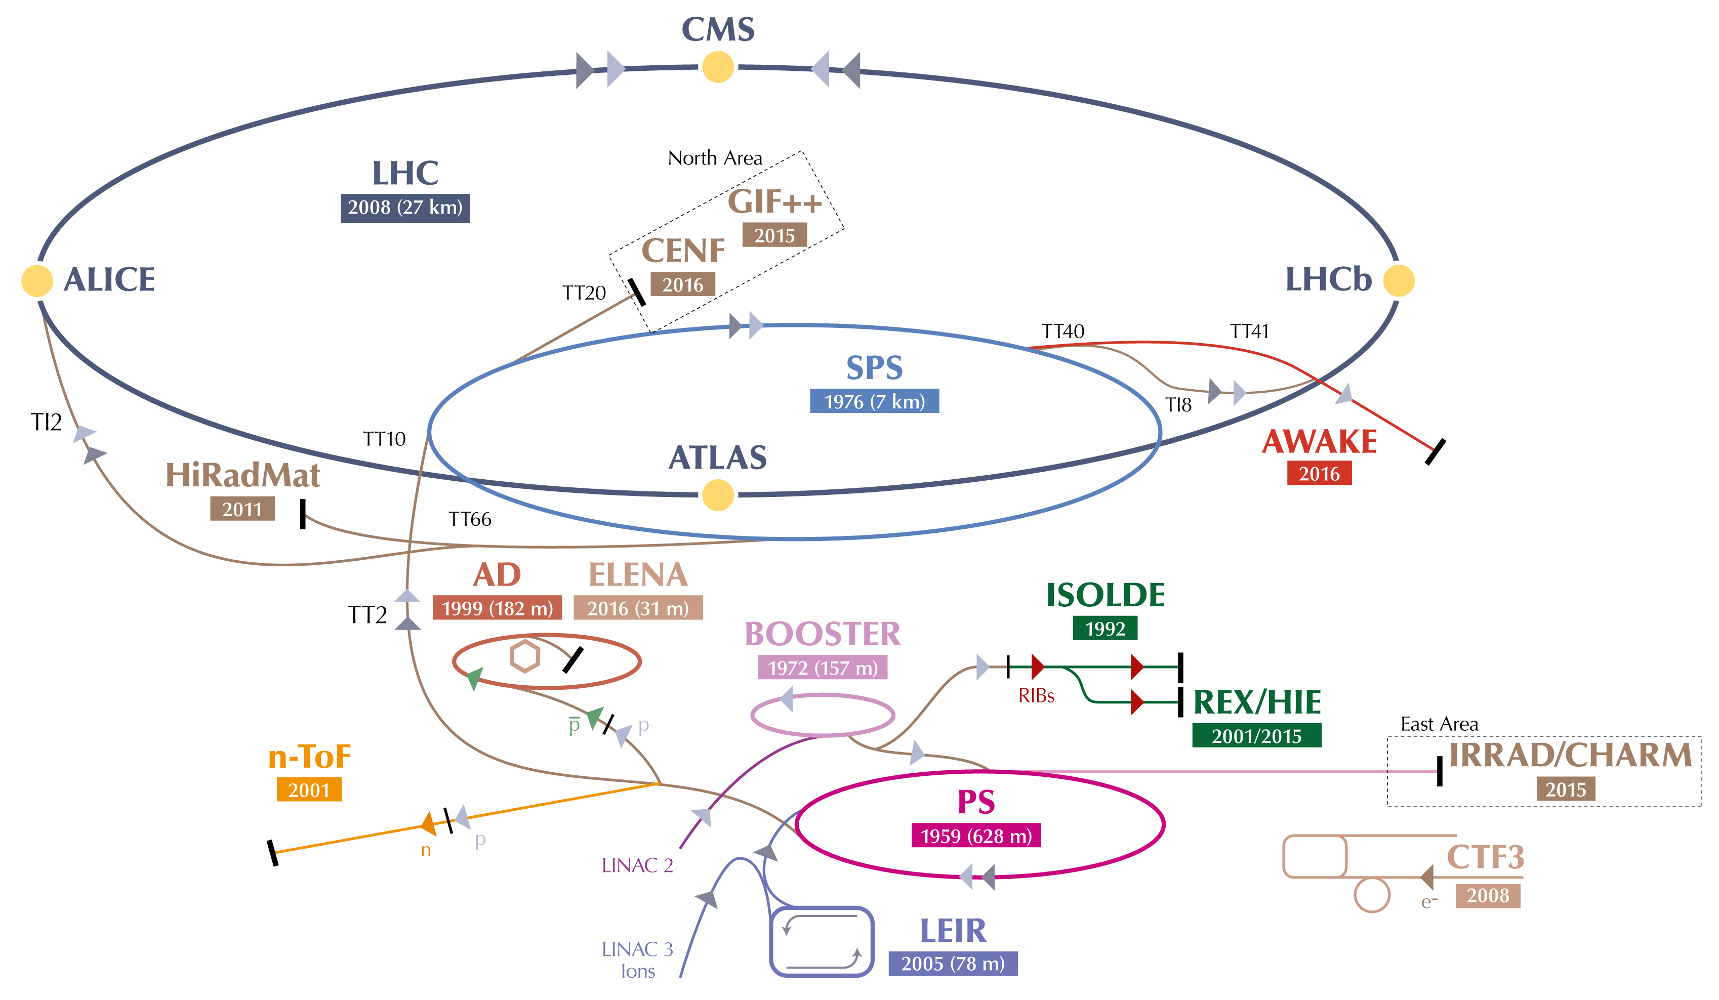
\includegraphics[width=.9\textwidth]{figs/detector/accelerator-complex-small}
  \caption[The CERN accelerator complex.  For LHC collisions, protons are accelerated by the Linac 2 (purple), the PSB (light purple), the PS (magenta), and the SPS (light blue) before entering the LHC ring (dark blue).]{The CERN accelerator complex.  For LHC collisions, protons are accelerated by the Linac 2 (purple), the PSB (light purple), the PS (magenta), and the SPS (light blue) before entering the LHC ring (dark blue)~\cite{2016.accelerator-image}.}
  \label{fig:detector_accelerator_complex}
\end{figure}

In addition to a high center of mass energy, the LHC must also deliver enough data to measure rare processes.
The amount of data collected is measured in terms of \emph{luminosity}.
The instantaneous luminosity $\mathcal{L}$ is defined in terms of the number of events per second $\deriv{R}{t}$ and the production cross section $\sigma_p$:
\begin{equation}
  \mathcal{L} = \frac{1}{\sigma_p}\deriv{R}{t}
  \label{eq:inst_lumi}
\end{equation}
The calculation itself can be quite tricky, as it depends on a number of factors including the number of particles per bunch, the spread of the beam, and the crossing angle of the beams~\cite{2006.lumi}.

The LHC was originally designed to operate at an instantaneous luminosity of $1.0\times 10^{34}~\textrm{cm}^{-2}\textrm{s}^{-1}$; however, this number was exceeded by the end of the 2016 data taking period, with a peak luminosity of $1.38\times 10^{34}~\textrm{cm}^{-2}\textrm{s}^{-1}$.
By the end of Run 2 in December 2018, the LHC was running at more than twice the design luminosity~\cite{2019.atlas-lumi-plots}.
The instantaneous luminosity of proton-proton collisions as a function of time in 2015 and 2016 are shown in Figure~\ref{fig:detector_instantaneous_lumi}.

The total amount of data collected is reported in terms of \emph{integrated} luminosity, which is simply the time integral of the instantaneous luminosity.
By the end of Run 2 (2015-2018), approximately $140~\textrm{fb}^{-1}$ of $13\tev$ data collected by the ATLAS detector is available for physics, as shown in Figure~\ref{fig:atlas_integrated_lumi}.
The $36.1~\textrm{fb}^{-1}$ collected during the first two years (2015 and 2016) is used for the analysis later in this thesis.

\begin{figure}[htbp]
  \centering
  \begin{subfigure}[b]{.48\textwidth}
    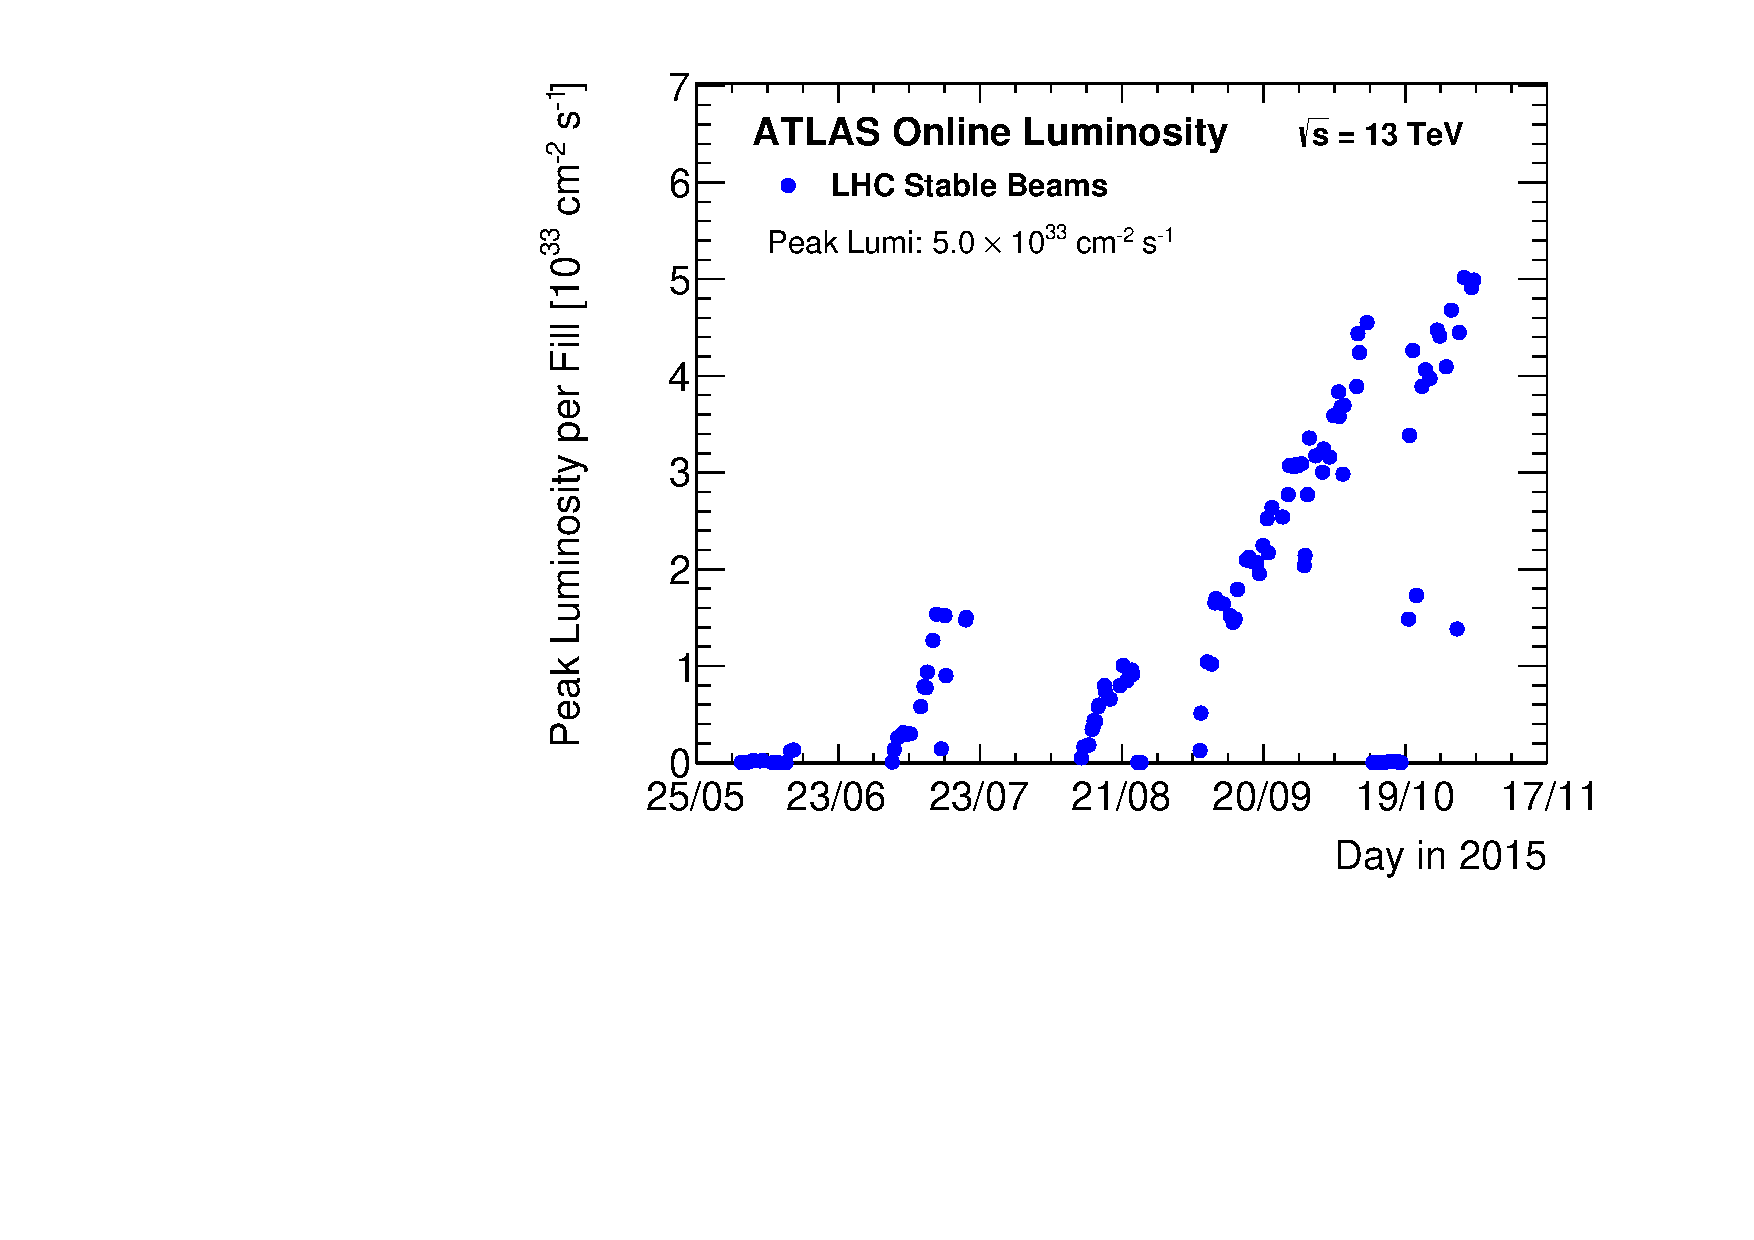
\includegraphics[width=\textwidth]{figs/detector/peakLumiByFill2015}
    \caption{2015}
  \end{subfigure}
  \begin{subfigure}[b]{.48\textwidth}
    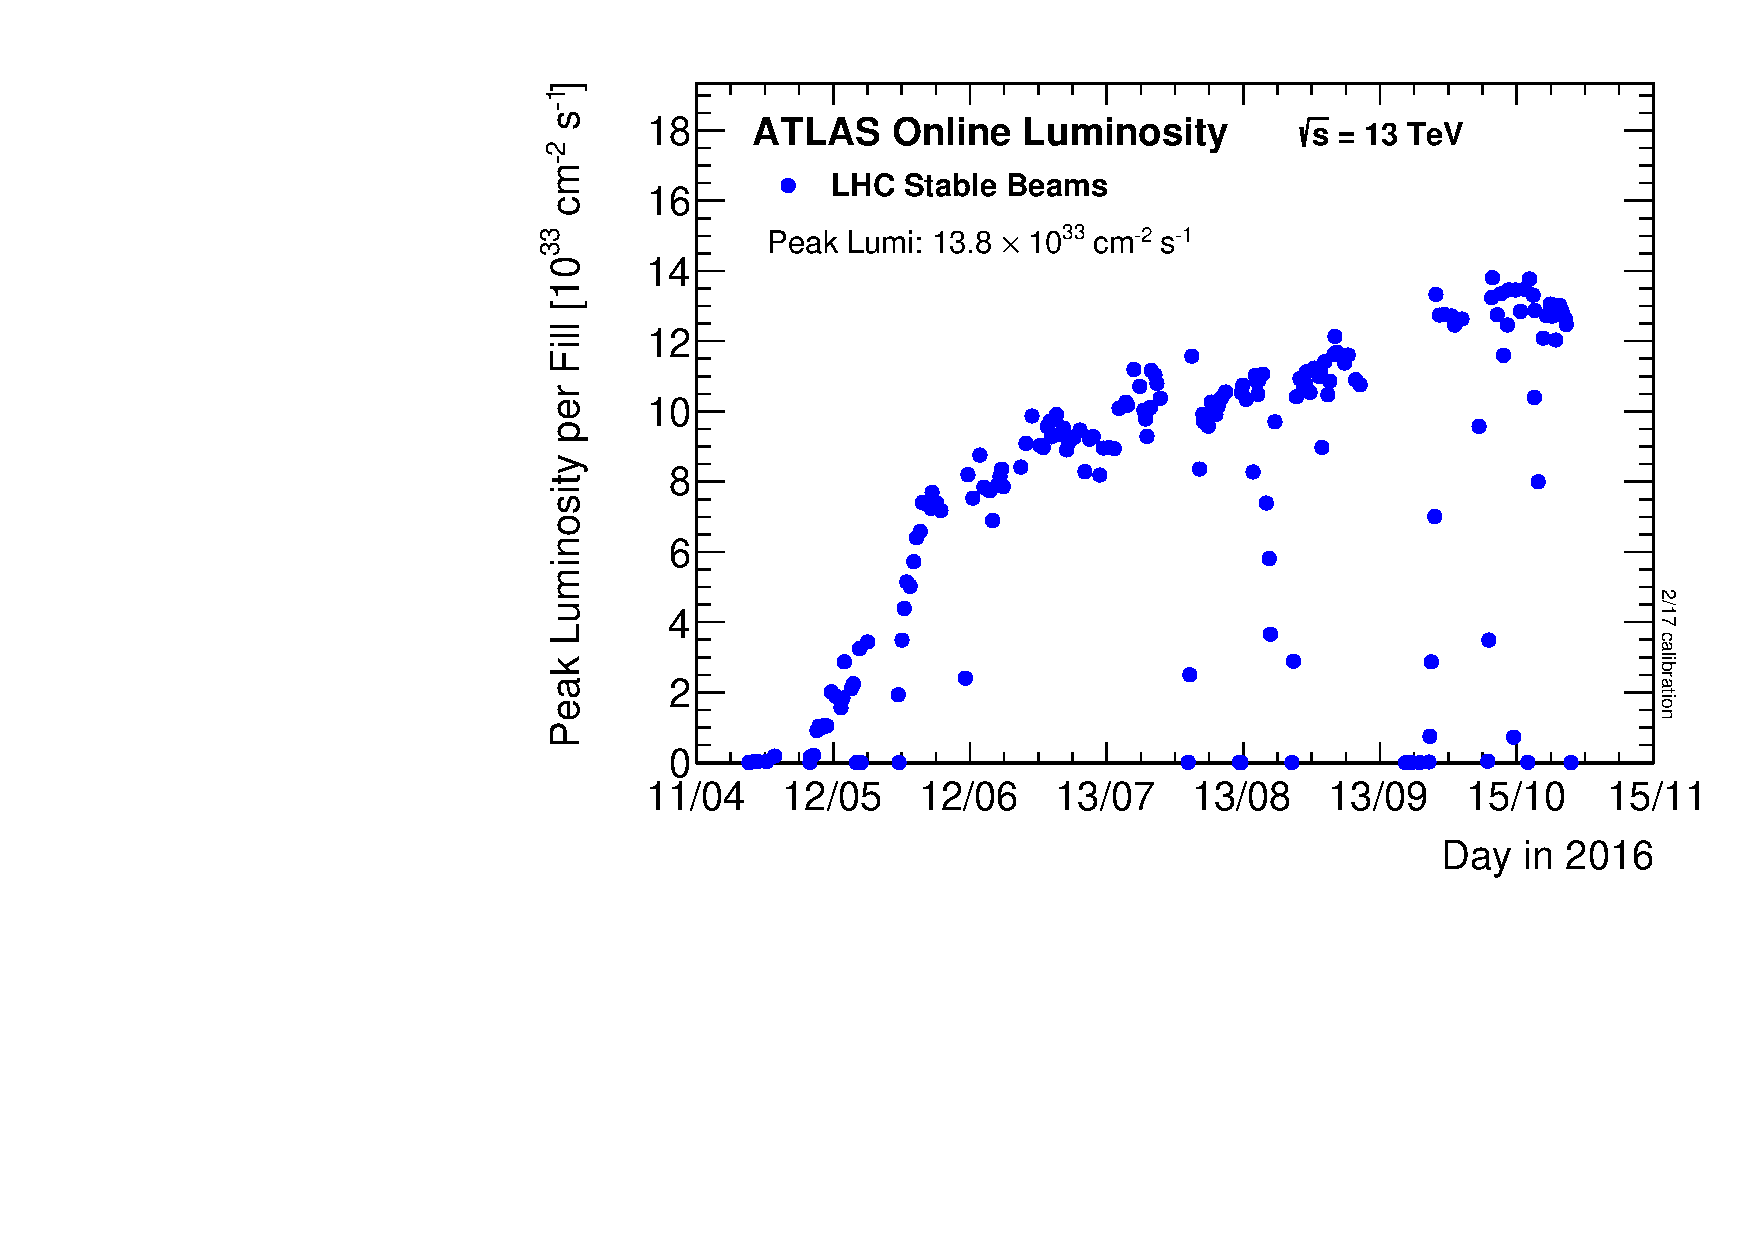
\includegraphics[width=\textwidth]{figs/detector/peakLumiByFill2016}
    \caption{2016}
  \end{subfigure}
  \caption[Peak instantaneous luminosity delivered to ATLAS during $13\tev$ $pp$ data taking as a function of time.]{Peak instantaneous luminosity delivered to ATLAS during $13\tev$ $pp$ data taking as a function of time~\cite{2019.atlas-lumi-plots}.}
  \label{fig:detector_instantaneous_lumi}
\end{figure}

\begin{figure}
  \centering
  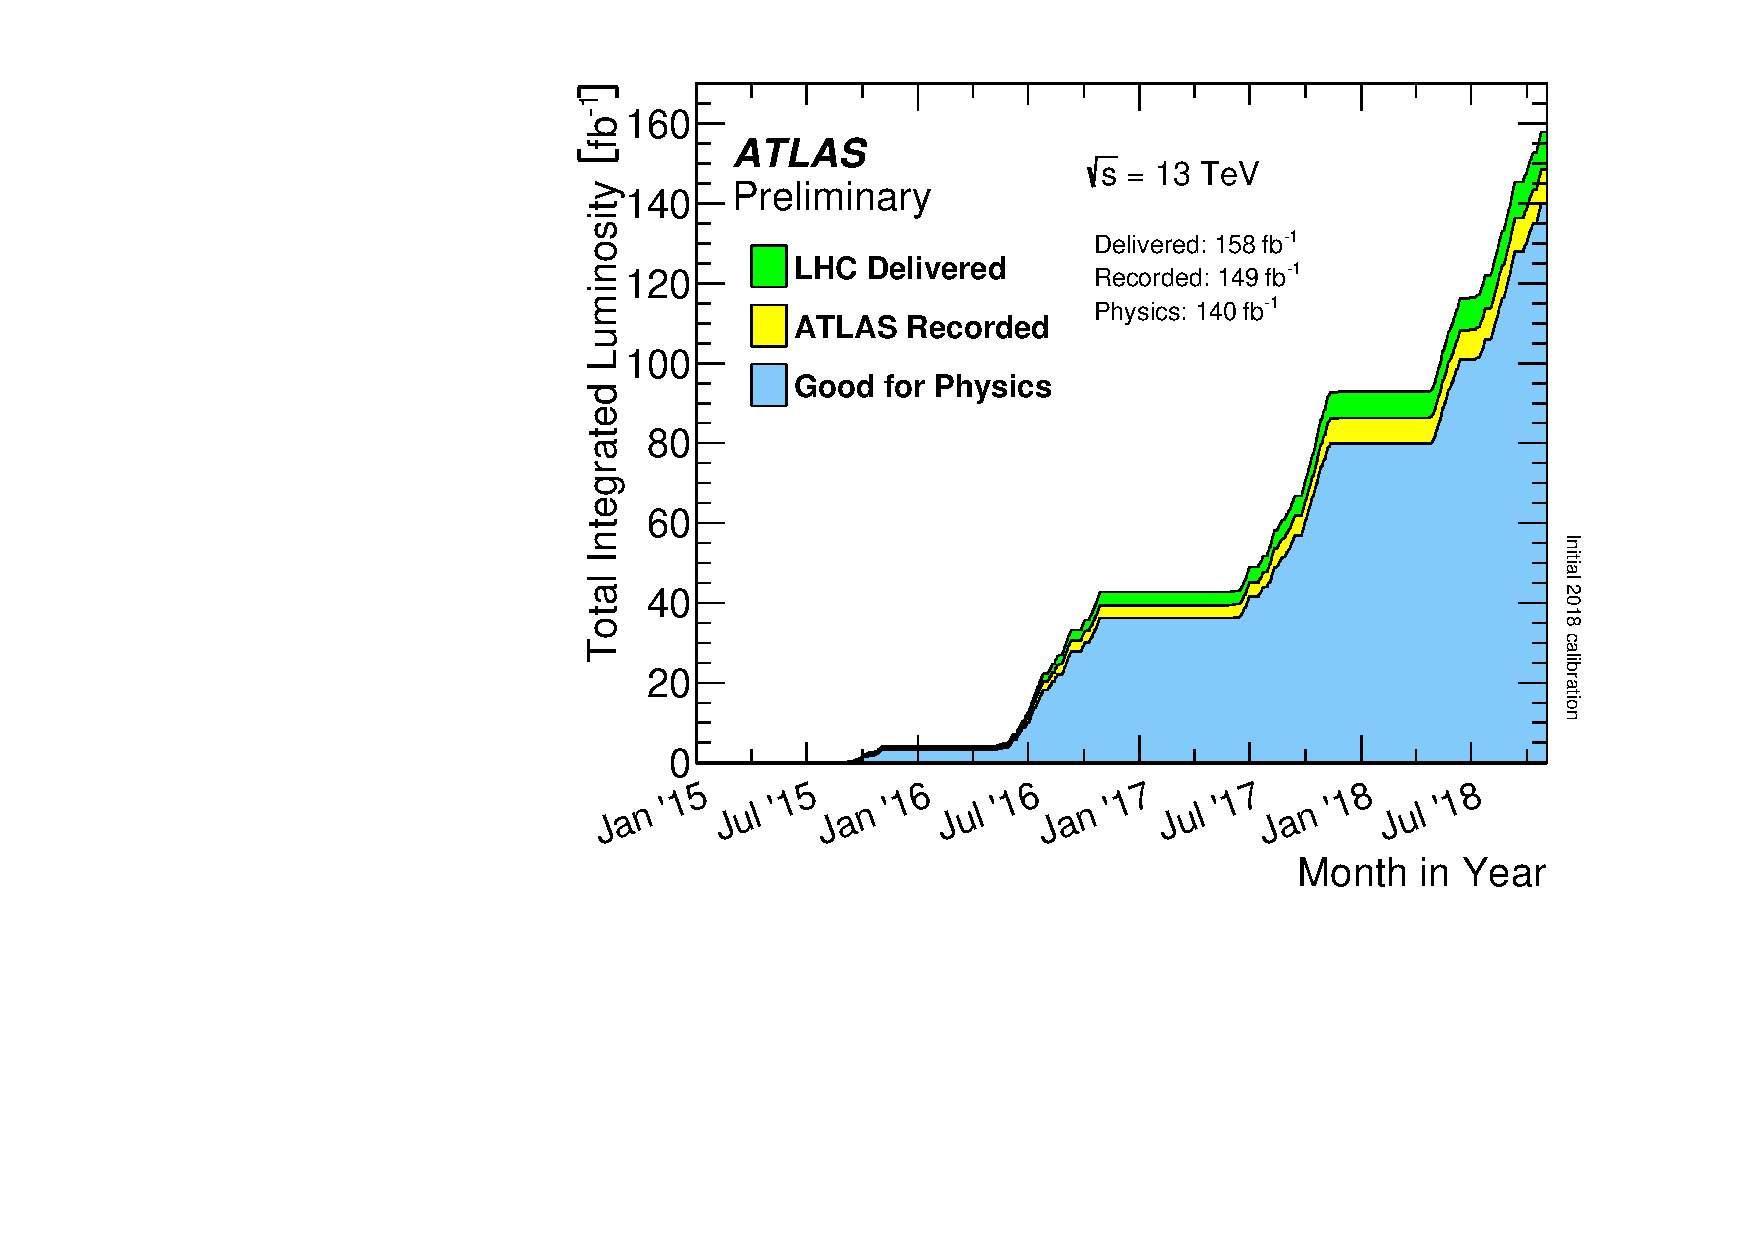
\includegraphics[width=.6\textwidth]{figs/detector/intLumiVsTimeRun2}
  \caption[Integrated luminosity collected by ATLAS as a function of time at $13\tev$ from 2015-2018.]{Integrated luminosity collected by ATLAS as a function of time at $13\tev$ from 2015-2018~\cite{2019.atlas-lumi-plots}.}
  \label{fig:atlas_integrated_lumi}
\end{figure}

Due to the high instantaneous luminosity, more than one $pp$ interaction occurs in a single bunch crossing, referred to as \emph{pileup}.
During the 2016 data taking campaign, the average number of interactions per bunch crossing $\textless\mu\textgreater$ was approximately 24 but has increased to upwards of 37 in 2017 and 2018~\cite{2019.atlas-lumi-plots}.
Figure~\ref{fig:detector_pileup} contains the average $\mu$ for the 2015-2016 data set used for analysis in this thesis.
The high pileup is a challenge for accurately reconstructing an individual collision.

\begin{figure}
  \centering
  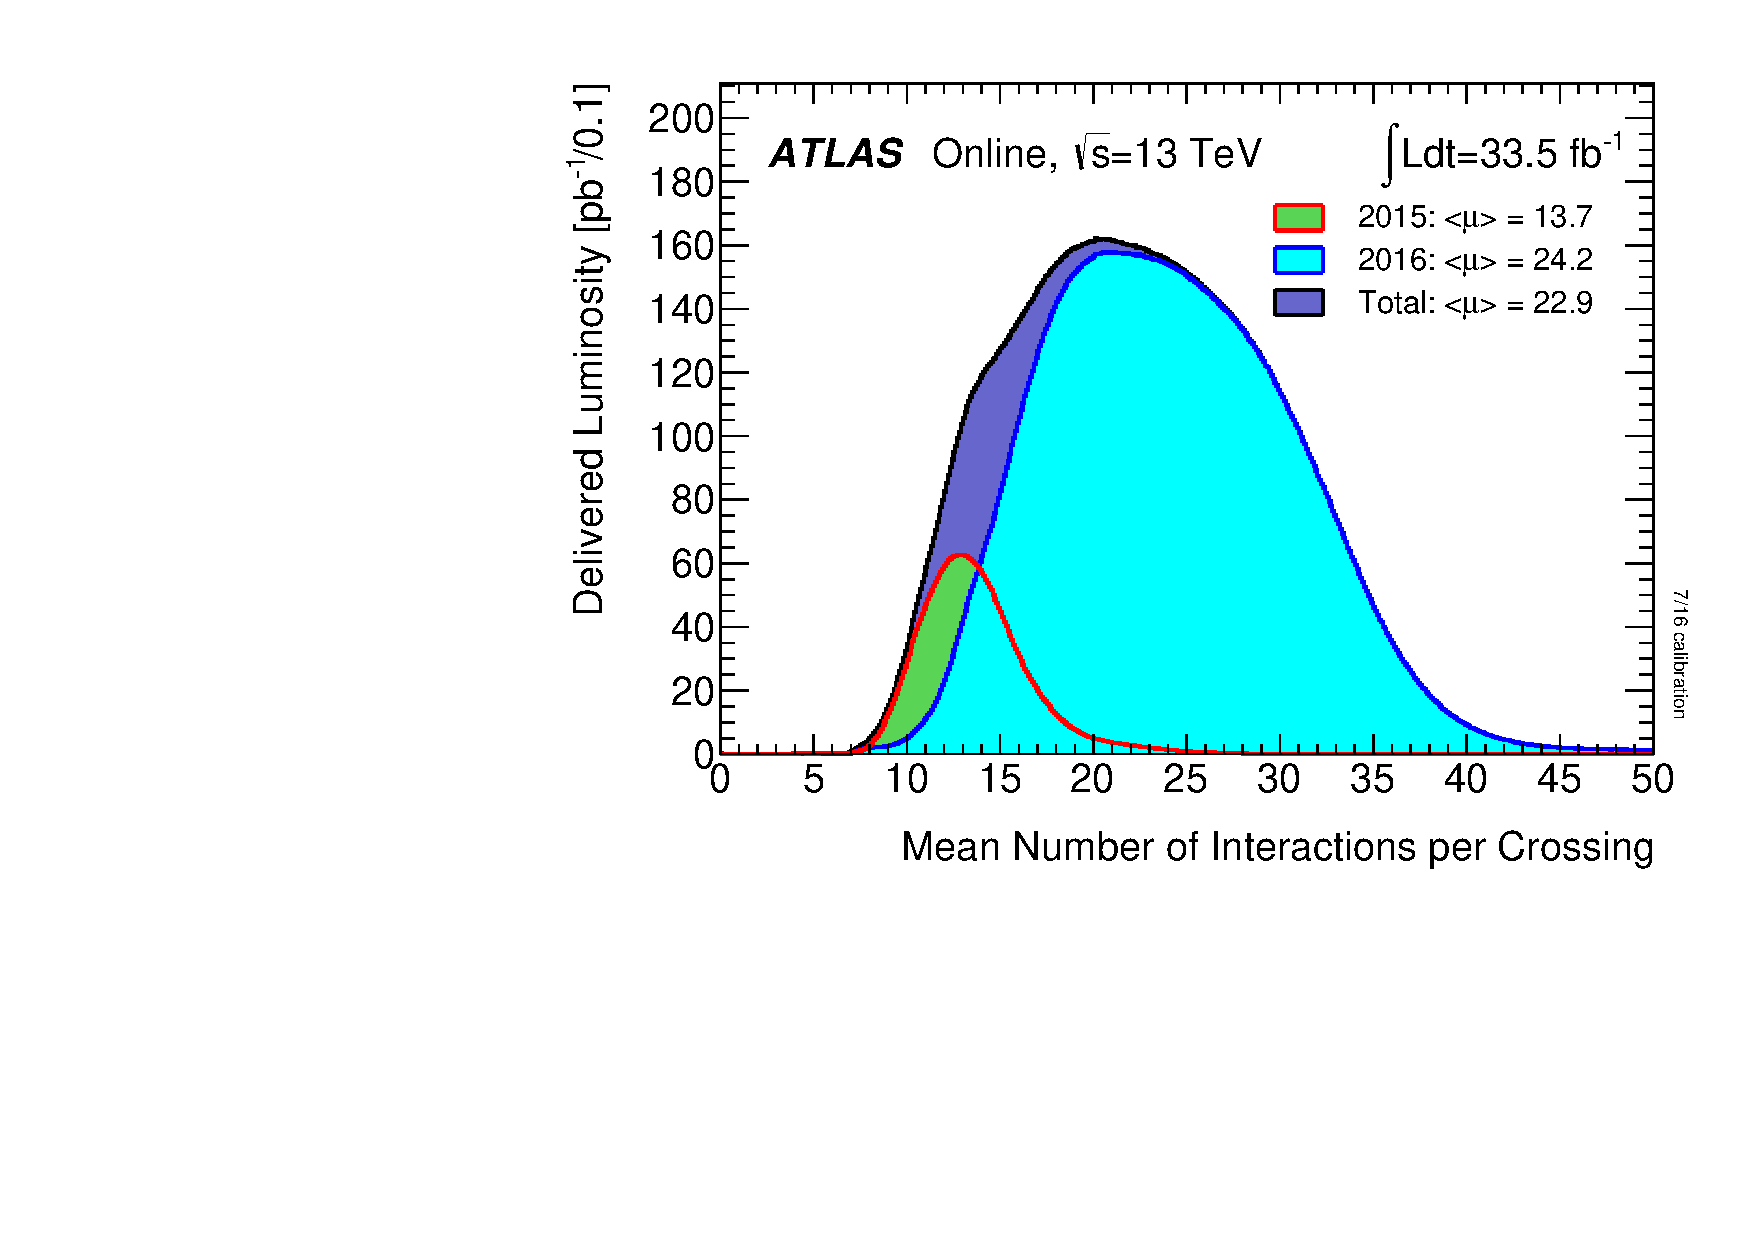
\includegraphics[width=.6\textwidth]{figs/detector/meanInteractionsPerCrossing}
  \caption[Distribution of the mean number of interactions per bunch crossing for the 2015 and 2016 $pp$ collision data at $13\tev$.]{Distribution of the mean number of interactions per bunch crossing for the 2015 and 2016 $pp$ collision data at $13\tev$~\cite{2019.atlas-lumi-plots}.}
  \label{fig:detector_pileup}
\end{figure}
